\chapter{Επαλήθευση Λειτουργίας και Αποτελέσματα} % Main chapter title
\label{chap:Chapter6}

% \epigraph{”Testing a product is a learning process"}{\textit{Brian Mahick}}
\epigraph{”Η διαδικασία δοκιμών ενός συστήματος είναι μία διαδικασία εκμάθησης''}{\textit{Brian Mahick}}

Σε αυτό το σημείο περιγράφονται οι ενέργειες που ακολουθήθηκαν, προκειμένου να επαληθευτεί η απόδοση του συστήματος.
Η διαδικασία δοκιμών χωρίστηκε σε τρία στάδια. Το πρώτο, το οποίο γινόταν σε indoor περιβάλλον ταυτόχρονα με την υλοποίηση του συστήματος
ώστε να επαληθευτεί η δυνατότητα εντοπισμού της μπάλας σε κάθε frame του feed της κάμερας\footnote{Βίντεο από την διαδικασία μπορεί να βρεθεί \cite{experiment-1-video}}. Την δεύτερη
που αποτελεί το κομμάτι δοκιμών ενός μεμονωμένου node σε outdoor scenarios για το localization στο image plane του αντικειμένου με βάση την μέθοδο εντοπισμού που επιλέχθηκε\footnote{
Βίντεο από την διαδικασία μπορεί να βρεθεί \cite{experiment-2-video}}. Τελευταίο κομμάτι ήταν η δοκιμή ολόκληρου του συστήματος.

Στην συνέχεια του κεφαλαίου, δίνονται αναλυτικά στοιχεία για την δεύτερη και τρίτη φάση δοκιμών και όχι για την πρώτη, καθώς περιλαμβάνονται σε αυτές μετρικές της πρώτης. Ενώ, για την ανίχνευση του object στο εκάστοτε καρέ χρησιμοποιείται η διαδικασία με τον HSV μετασχηματισμό (βλ. \Sect{hsv-detection-sec}).

Ο λόγος επιλογής της HSV μεθόδου στην συγκεκριμένη εργασία είναι ότι μπορεί να παρέχει ικανοποιητική απόδοση όντως πρώτη γενιά του συστήματος - με μικρές σχετικά ανάγκες επεξεργασίας - παρόλα αυτά, κύριο αρνητικό της είναι η ανάγκη πριν την χρήση του συστήματος να πραγματοποιηθεί calibration. Για
να ξεπεραστεί αυτός ο περιορισμός - ακολουθώντας την ίδια προσέγγιση υλοποίησης - αρκεί μελλοντικά να αντικατασταθεί η κάμερα με μία Infrared (\Abbr{IR}).

\section{Επαλήθευση λειτουργίας μεμονωμένου node}

\subsection{Περιβάλλον δοκιμών}
Για την επαλήθευση λειτουργίας του μεμονωμένου κόμβου, η διαδικασία που ακολουθήθηκε είναι η εξής. 
Χρησιμοποιήθηκαν δύο αντικείμενα, το υπό έλεγχο σύστημα - \Fig{node-testing-env} (a) - το οποίο κατά όλη την διάρκεια του πειράματος ήταν στατικό σε συγκεκριμένο σημείο, και το κινούμενο αντικείμενου (η κίτρινη μπάλα), η θέση του οποίου έγινε προσπάθεια κάθε χρονική στιγμή να εκτιμηθεί - \Fig{node-testing-env} (b).   

\begin{figure} [H]
	\centering
	% -----------------
    \begin{minipage}{.5\textwidth}
      \centering
      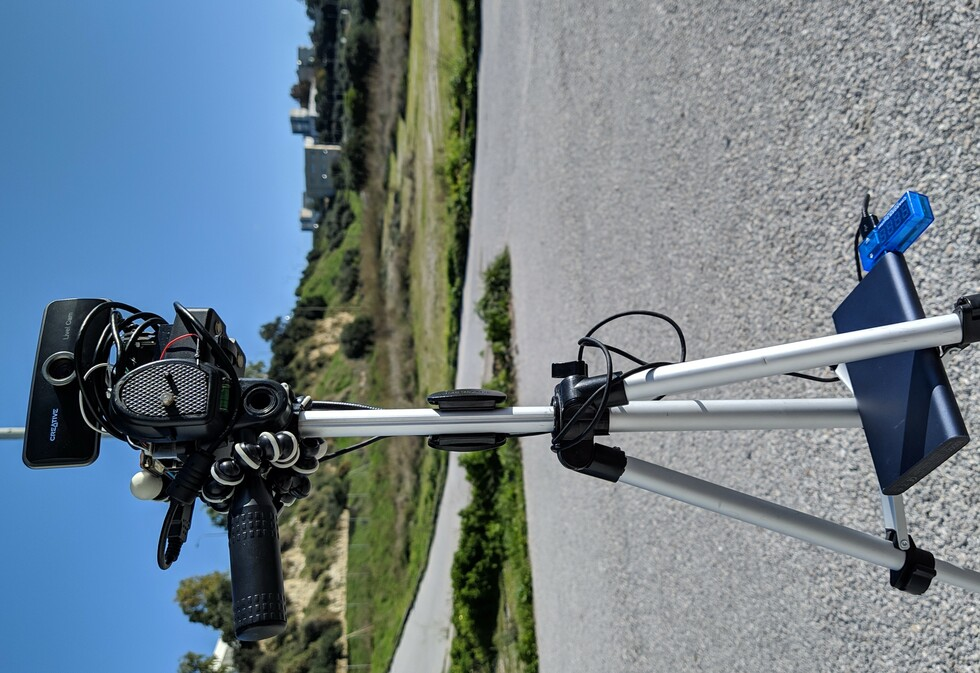
\includegraphics[width=\linewidth, angle =-90]{../Images/Experiments-Results/node.jpg} \\ \vspace{0.1cm}
      {(a) Υπό έλεγχο σύστημα (Node) το οποίο τροφοδοτείται από powerbank κατά την διάρκεια πειραμάτων}
    \end{minipage}%
    % -----------------
    \begin{minipage}{.5\textwidth}
      \centering
      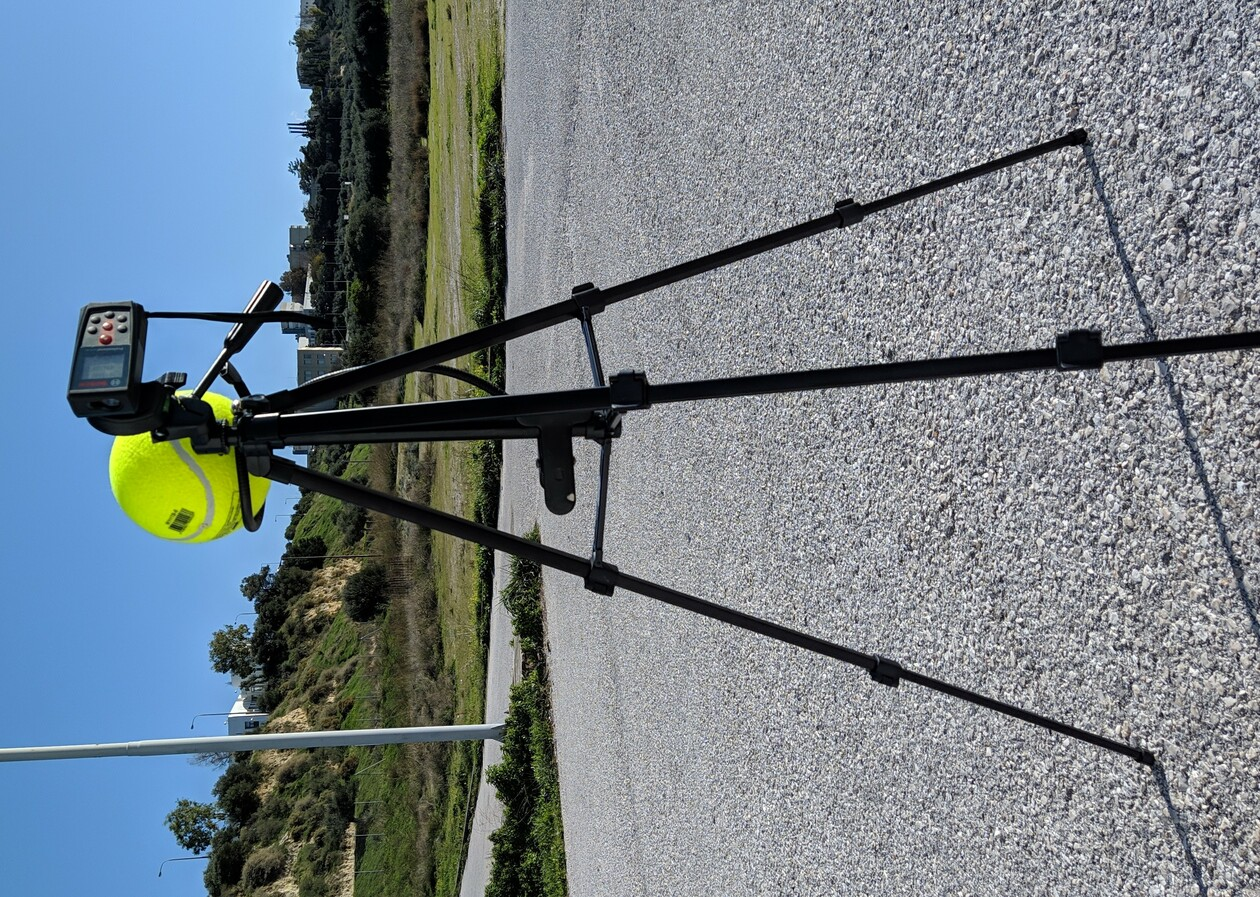
\includegraphics[width=\linewidth, angle =-90]{../Images/Experiments-Results/testing.jpg}\\ \vspace{0.1cm}
      {(b) Κινούμενο αντικείμενο εκτίμησης θέσης μαζί με το όργανο μέτρησης απόστασης }
	\end{minipage}
	% -----------------
    \hfill \break
    \decoRule
    \CaptionBasedwithURL{Εξοπλισμός που χρησιμοποιήθηκε στην πρώτη εξωτερική πειραματική φάση} 
    \label{fig:node-testing-env}
\end{figure}

Τα δύο αυτά αντικείμενα τοποθετήθηκαν το ένα απέναντι από το άλλο όπως φαίνεται στην \Fig{single-test-bench-side-view}, και πάρθηκαν μετρήσεις απόστασης για διαφορετικές γωνίες όπως φαίνεται στην 
\Fig{single-test-bench-angles}. Ταυτόχρονα, το σύστημα κατά την διάρκεια της διαδικασίας, ήταν σε πλήρη λειτουργία, και πραγματοποιούσε ανίχνευση και εκτίμηση της απόστασης του αντικειμένου από την κάμερα. Στη
\Sect{expe-single-3d} παρουσιάζονται τα πειραματικά αποτελέσματα των μετρήσεων αυτής της διαδικασία, ενώ στη 
\Sect{single-expe-system} παρουσιάζονται οι ανάγκες λειτουργίας από την σκοπιά του ε\-νσω\-μα\-τω\-μέ\-νου συστήματος.

\FigCaptLabelBasedURL{../Images/Experiments-Results/side.jpg}
{Χωρική τοποθέτηση του υπό ελέγχου συστήματος και αντικειμένου εκτίμησης θέσης}%
{single-test-bench-side-view}%
<0.8>

\FigCaptLabelBasedURL{../Images/Experiments-Results/testbench.png}
{Αναπαράσταση των θέσεων στις οποίες έγιναν οι μετρήσεις του πειράματος}%
{single-test-bench-angles}%
<0.6>

Όπως φαίνεται στην \Fig{node-testing-env} (b), το object το οποίο πρόκειται να εντοπίσουμε βρίσκεται σε τρίποδο, για μεγαλύτερη ευκολία των μετρήσεων, ενώ στο πλάγιο μέρος γίνεται διακριτό το όργανο που χρησιμοποιήθηκε για τον υπολογισμό της απόστασης μεταξύ των δύο αντικειμένων. Το όργανο αυτό είναι το laser range finder της Bosch GLM 40 - \Fig{bosch-range-estimator} - με δυνατότητες μέτρησης $0.15-40.00 m$ και απόκλιση μετρήσεων $\pm1.5mm$

Για τον υπολογισμό των διάφορων γωνιών από τις οποίες θα γινόντουσαν μετρήσεις, χρησιμοποιήθηκε το όργανο μέτρησης γωνιών όπως φαίνεται στην \Fig{single-test-bench-top-view}. Ενώ οι μετρήσεις που στην συνέχεια θα αναγερθούν αφορούν δεδομένα από γωνίες [$-20\si{\degree},-10\si{\degree},~0\si{\degree},~10\si{\degree},~20\si{\degree}$]\footnote{Λόγω του διαφορετικού ύψους μεταξύ της θέσης που μετρήθηκαν οι γωνίες και της κάμερας, δεν είναι οι ίδιες με αυτές που ανιχνεύονται στο x άξονα της εικόνας} και αποστάσεις μέτρησης ανά 50cm μέχρι τα 5m (εκτός από την κεντρική ευθεία στην οποία έγιναν μετρήσεις μέχρι περίπου τα 8m).

\FigCaptLabelBasedURL{../Images/Experiments-Results/glm40.jpg}
{Το ψηφιακό λέιζερ μέτρησης απόστασης που χρησιμοποιήθε (Bosch GLM 40)}%
{bosch-range-estimator}%
<0.4>%
(https://www.howetools.co.uk/bosch-glm-40-aaa-batteries-laser-range-finder)

\FigCaptLabelBasedURL{../Images/Experiments-Results/node-top-view.jpg}
{Υπολογισμός των γωνιών με χρήση εργαλείου μέτρησης γωνίας}%
{single-test-bench-top-view}%
<0.9>

% -------------------------------------------------------------
\subsection{Απόδοση του συστήματος} \label{sec:single-expe-system}

Πριν αναφερθούν τα δεδομένα που συλλέχθηκαν ως προς την απόδοση του συστήματος, θα αναφερθούν κάποια από τα 
χαρακτηριστικά λειτουργίας του. Η υλοποίηση του συστήματος έγινε σε C++. Δημιουργήθηκαν συνεπώς Function-like macros για εξαγωγή και αποθήκευση χρήσιμων πληροφοριών του συστήματος. Οι πληροφορίες που συλλέχθηκαν, αναφέρονται σε αυτήν την ενότητα, και σχετίζονται με τις επεξεργαστικές και ενεργειακές ανάγκες του συστήματος, η μνήμη μου χρειάζεται για να λειτουργήσει, και άλλες σημαντικές πληροφορίες.

Πρώτη από αυτές τις πληροφορίες είναι οι επεξεργαστικές ανάγκης του, όπου στην \Fig{cpu-usage-experiment-example}
φαίνονται τα δεδομένα που συλλέχθηκαν κατά την διάρκεια ενός από τα πειράματα. 

\FigCaptLabelBasedURL{../Images/Experiments-Results/raspberry-exp-cpu.png}
{Επεξεργαστική ισχύς του συστήματος}%
{cpu-usage-experiment-example}%
<1>

Μία ακόμα χρήσιμη μετρική είναι αυτή της μνήμης που χρησιμοποιεί το σύστημα, στην \Fig{ram-usage-experiment-example}
παρουσιάζεται η συγκεκριμένη πληροφορία. Από αυτό το διάγραμμα μπορούμε να παρατηρήσουμε ότι για την συγκεκριμένη υλοποίηση το σύστημα δεν έχει μεγάλες ανάγκες μνήμης\footnote{Έχοντας αυτήν την πληροφορία, μπορούμε να μεταβούμε σε επιλογή Embedded Linux System με μικρότερη μνήμη, που σημαίνει μικρότερο κόστος ανά node συστήματος}.
\FigCaptLabelBasedURL{../Images/Experiments-Results/raspberry-exp-ram.png}
{Ανάγκες μνήμης του συστήματος}%
{ram-usage-experiment-example}%
<1>

Το σύστημα αυτό σχεδιάζεται, με γνώμονα μελλοντικά να χρησιμοποιηθεί σε drones, συνεπώς οι ενεργειακές απαιτήσεις του είναι σημαντικές. Για αυτό τον λόγο ε\-ξά\-χθη\-καν και δεδομένα σχετικά με την κατανάλωση του συστήματος\footnote{Στις συγκεκριμένες γραφικές, μέχρι το 80s το σύστημα είναι σε idle mode, ενώ από εκεί και έπειτα είναι σε πλήρη λειτουργία} - \Fig{power-usage-experiment-example}. Με την μέγιστη κατανάλωση που παρατηρήθηκε από τροφοδοσία μέσω power bank κατά την διάρκεια δοκιμών είναι τα 10Watt, ενώ τάση τροφοδοσίας είναι τα 5Volt.
\FigCaptLabelBasedURL{../Images/Experiments-Results/raspberry-exp-power.png}
{Ενεργιακές απαιτήσεις συστήματος}%
{power-usage-experiment-example}%
<1>

Σημαντικός παράγοντας της απόδοσης ενός επεξεργαστή, είναι η θερμοκρασία του, καθώς αν είναι αυξημένη μπορεί η απόδοση να μειωθεί λόγω thermal throttling. Για αυτό συλλέχθηκε επίσης πληροφορία για την θερμοκρασία του επεξεργαστή - \Fig{temp-usage-experiment-example}. 
\FigCaptLabelBasedURL{../Images/Experiments-Results/raspberry-exp-temp.png}
{Θερμοκρασίες συστήματος έχοντας σε χρήση το fan του breakout board}%
{temp-usage-experiment-example}%
<1>

Ενώ τελευταία, αλλά εξίσου σημαντική μετρική, είναι ο υπολογισμός του χρόνου που χρειάζεται το σύστημα ανίχνευσης του αντικειμένου, για κάθε δευτερόλεπτο χρήσης του συστήματος, και παρουσιάζεται στην \Fig{hsv-calc-dur-experiment-example}.
\FigCaptLabelBasedURL{../Images/Experiments-Results/raspberry-exp-hsv-dur.png}
{Χρόνος του object detection μέσα σε κάθε δευτερόλεπτο χρήσης του συστήματος}%
{hsv-calc-dur-experiment-example}%
<1>

%----------------------------------------------------------------------

\subsection{Λαμβανόμενα δεδομένα και απεικόνιση} \label{sec:expe-single-3d}

Πριν αναφερθούν τα δεδομένα που λήφθηκαν κατά το πείραμα, είναι σημαντικό να γίνει κατανοητή η εξάρτηση pixel-απόστασης της σχέσης \EqNum{distance-from-object-pixels} που αναλύθηκε στο προηγούμενο κεφάλαιο και χρησιμοποιείται για το range estimation του αντικειμένου.

Η \Fig{pixel-dist-rel} παρουσιάζει την παραπάνω αναλογία, για τις παραμέτρους της κάμερας που χρησιμοποιήθηκε, σε αναλύσεις 1280x720 pixels.

\FigCaptLabelBasedURL{../Images/Experiments-Results/pixels-dist-rel.png}
{Εξάρτηση του μεγέθους του αντικειμένου σε pixel με απόσταση αντικειμένου από την κάμερα}%
{pixel-dist-rel}%
<1>

Αυτό που μπορούμε να παρατηρήσουμε είναι, ότι δεν είναι γραμμική. Όμως, μπορεί να προσεγγιστεί σε ένα υποσύνολο του πεδίο ορισμού της, με γραμμικό τρόπο. Αυτό σημαίνει ότι για σχετικά μεγάλες ακτίνες η μεταβολή σε pixel επιφέρει μικρές με\-τα\-βο\-λές στην απόσταση, ενώ για μικρές ακτίνες επιφέρει μεγάλες μεταβολές της απόστασης. 

Για λόγους πληρότητας θα δοθούν τρία παραδείγματα. Σε πολύ μικρές ακτίνες - λόγου χάρη για αντικείμενο ακτίνας 10 pixel - η εκτιμώμενη απόσταση είναι 12.4m, ενώ, αν το αντικείμενο εκτιμούσαμε ότι είχε ακτίνα 11 pixel, τότε η απόσταση θα ήταν 11.27m. Ως αποτέλεσμα, σε αυτήν την περίπτωση το 1 pixel σφάλματος του αντικειμένου στο image plane να καταλήγει σε 1.13m σφάλματος της εκτιμώμενης απόστασης στον φυσικό κόσμο. Για λίγο μεγαλύτερες ακτίνες, όπως για 50 pixel, η εκτιμώμενη απόσταση είναι 2.48m. Αν όμως για αυτή την ακτίνα του αντικείμενου είχαμε σφάλμα 1 pixel - δηλαδή μέτρηση 51 pixel - τότε η εκτιμώμενη απόσταση θα ήταν τα 2.43m, με τελικό σφάλμα τα 5cm σε αυτήν την περίπτωση. Τέλος, σε αρκετά μεγαλύτερες ακτίνες, με τα 100 pixel ως αναφορά, έχουμε εκτιμώμενη α\-πό\-στα\-ση τα 1.24m, ενώ, σε περίπτωση που η ακτίνα μας έχει 1 pixel διαφορά από την πραγματικότητα - δηλαδή έστω 101 pixels - και τα 1.22m εκτιμώμενη απόσταση, καταλήγουμε σε 2cm σφάλμα. Αυτό που βγαίνει ως συμπέρασμα από αυτήν την σχέση είναι ότι το τελικό σφάλμα εκτίμησης είναι σε άμεση εξάρτηση με το ποσοστό του image plane που καταλαμβάνει το αντικείμενο σε αυτό. 

Αφού έχει γίνει ξεκάθαρος αυτός ο περιορισμός, θα αναφερθούν τα δεδομένα που λήφθηκαν κατά την διάρκεια του πειράματος, από το node.
Αρχικά, στην \Fig{raspberry-exp-node-view} παρουσιάζεται στιγμιότυπο της αντιληπτικής ικανότητας - μεμονωμένης χρονικής στιγμής - του node, μαζί με τα διάφορα στάδια ε\-πε\-ξε\-ργα\-σίας, σε συνδυασμό με post-processing τρισδιάστατη απεικόνιση της μπάλας σε σχέση με την κάμερα (κάτω δεξιά στην εικόνα).

\FigCaptLabelBasedURL{../Images/Experiments-Results/node-view.png}
{Αντιληπτική ικανότητα μεμονωμένου κόμβου κατά την διάρκεια των δοκιμών, σε συνδυασμό με τρισδιάστατη απεικόνιση της μπάλας}%
{raspberry-exp-node-view}%
<1>

Οι γραφικές - \Fig{dist-experiment-example} και \Fig{angles-usage-experiment-example} - παρουσιάζουν τα raw data για την α\-πό\-στα\-ση και γωνίες που συλλέχθηκαν κατά την διάρκεια του πειράματος. Με την βοήθεια αυτών, μπορεί ακόμα και να φανεί η διαδρομή που ακολουθήθηκε κατά την διάρκεια του πειράματος. Επίσης, παρατηρείται να είναι σε ένα αρκετά μεγάλο ποσοστό κοντά στην πραγματική διαδρομή, με πολύ καλή προ\-σέ\-γγι\-ση για τον ε\-ντο\-πι\-σμό του αντικειμένου (όπως θα φανεί στην συνέχεια). Για τις οποίες, είναι σημαντικό όμως να αναφερθεί ότι τα spikes αναπαριστούν σημεία όπου δεν είχε γίνει ακριβές detection του object.

\begin{figure}[H]
  \centering
  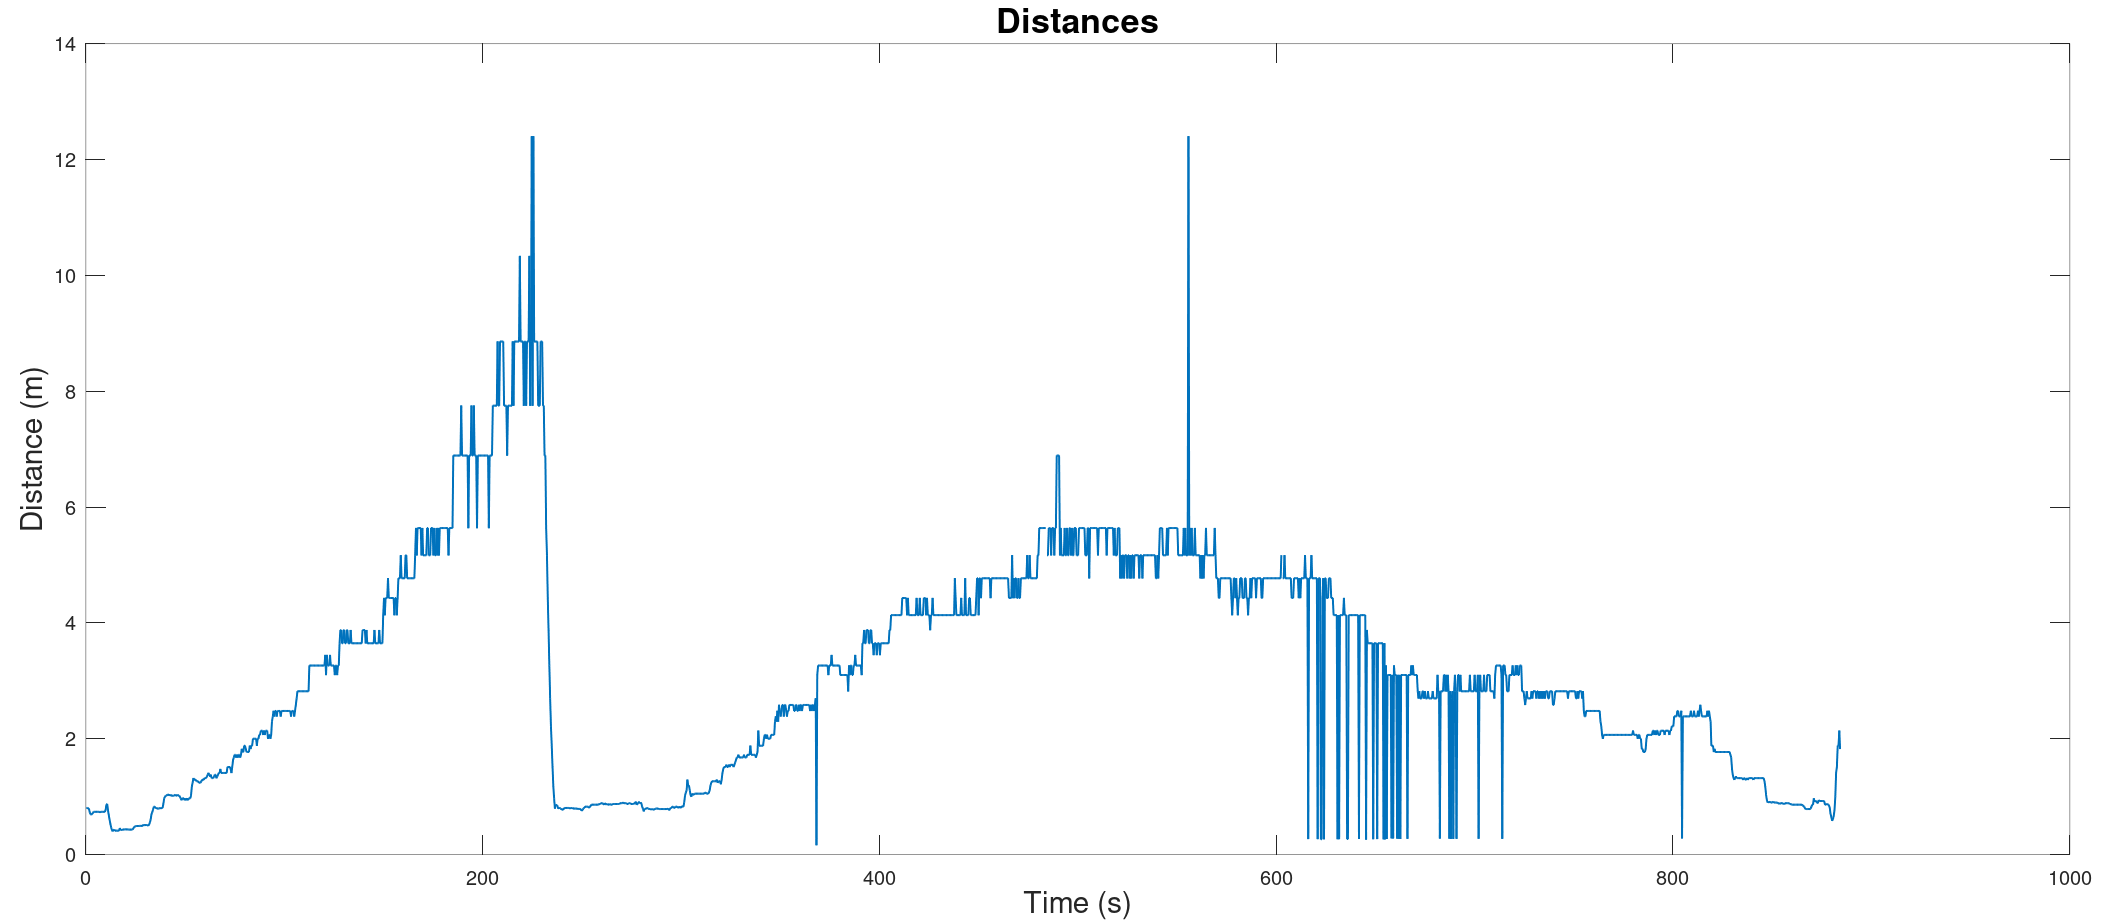
\includegraphics[width=\linewidth]{../Images/Experiments-Results/raspberry-exp-dist.png}
  \decoRule
  \caption[Εκτίμηση απόστασης για κάθε δευτερόλεπτο χρήσης του συστήματος]{Εκτίμηση απόστασης για κάθε δευτερόλεπτο χρήσης του συστήματος (για 3 από τις 5 ευθείες)}
  \label{fig:dist-experiment-example}
\end{figure}


\begin{figure}[H]
  \centering
  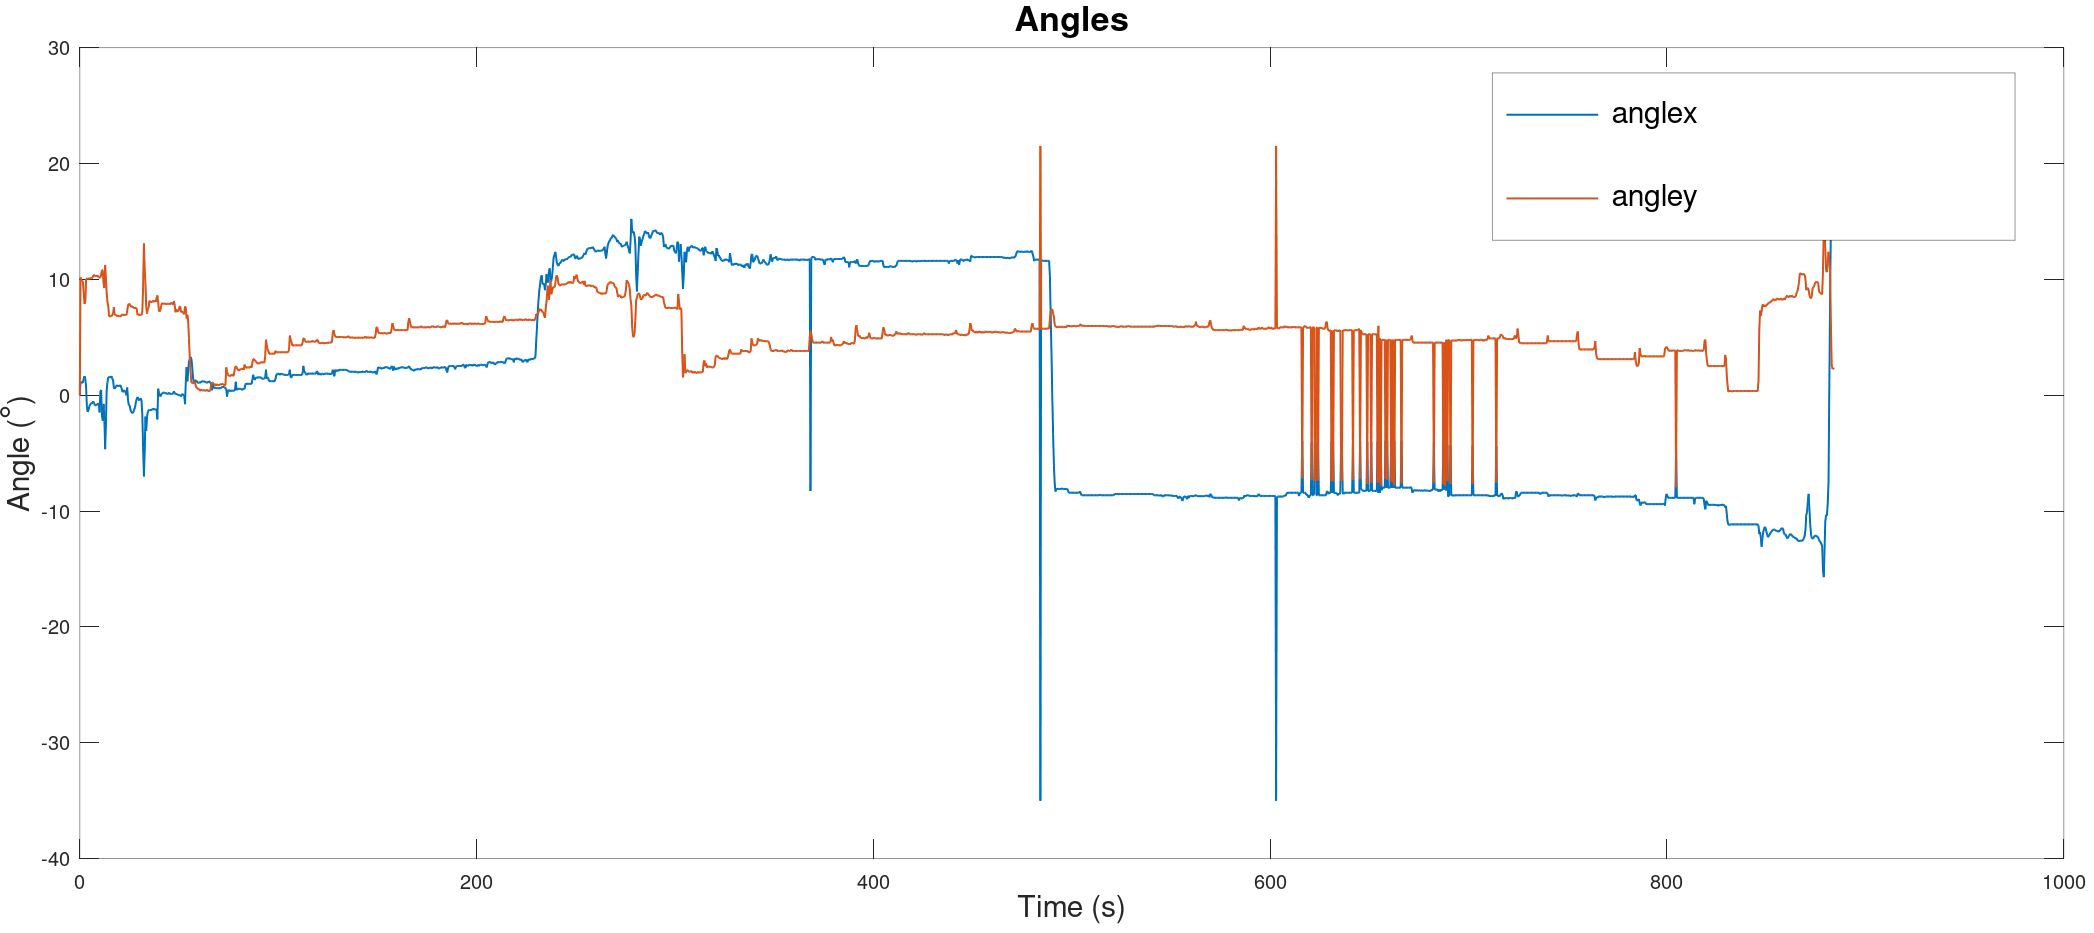
\includegraphics[width=\linewidth]{../Images/Experiments-Results/raspberry-exp-angles.png}
  \decoRule
  \caption[Εκτίμηση γωνιών στους άξονες x και y για κάθε δευτερόλεπτο χρήσης του συστήματος]{Εκτίμηση γωνιών στους άξονες x και y για κάθε δευτερόλεπτο χρήσης του συστήματος (για 3 από τις 5 ευθείες)}
  \label{fig:angles-usage-experiment-example}
\end{figure}

Με βάση τις δύο παραπάνω γραφικές, για την εκτίμηση απόστασης και γωνιών οι οποίες αποτελούν scalar τιμές, μπορούμε σε συνδυασμό - με απλή γεωμετρία - να αναπαραστήσουμε στο τρισδιάστατο χώρο όλες τις εκτιμήσεις για τις θέσης του αντικειμένου και να καταλήξουμε σε ένα vector θέσης ως προς την κάμερα. Αυτό γίνεται προσπάθεια να επιτευχθεί στην \Fig{obj-3d-repre}. Θεωρητικά θα μπορούσαμε μόνο με αυτόν τον τρόπο να εντοπίσουμε το αντικείμενο στον \Abbr{3D} χώρο, για λόγους α\-ξιο\-πι\-στίας όμως ωθούμαστε στον προσδιορισμό της θέσης από δεδομένα πολλαπλών κόμβων - από swarm - ώστε σε μία πιθανή αποστολή να μην έχουμε single point of failure. 

\FigCaptLabelBasedURL{../Images/Experiments-Results/raspberry-exp-obj-3d.png}
{Τρισδιάστατη απεικόνιση των μετρήσεων για 3 από τις 5 ευθείες}%
{obj-3d-repre}%
<1>

%----------------------------------------------------------------------

\section{Δεδομένα πολλαπλών κόμβων}
Όπως αναφέρθηκε και στη \Sect{GPS}, η λειτουργία του \Abbr{GPS} - τουλάχιστον σε αυτήν την φάση - ήταν για λόγους πληρότητας της υλοποίησης, ώστε να γίνει εύκολο το integration ενός \Abbr{GPS} με μικρότερο σφάλμα - όπως \Abbr{RTK} \Abbr{GPS} - σε μελλοντική υλοποίηση. Για αυτόν τον λόγο στην συνέχεια αναφερόμαστε σε καθορισμένων συντεταγμένων nodes.

%----------------------------------------------------------------------

\subsection{Διαδικασία λήψης δεδομένων} \label{sec:multiple-nodes-data-collection}
Στην συνέχεια πραγματοποιήθηκαν μετρήσεις από πολλαπλά σημεία (κόκκινα τε\-τρά\-γω\-να στο διάγραμμα) για το ίδιο αντικείμενο όπως παρουσιάζεται στην \Fig{multiple-nodes-positions}.
Με αυτόν τον τρόπο, για την ίδια θέση της μπάλας (με μαύρο χρώμα στο διάγραμμα) θα μπορούσε να προσομοιωθούν - σε ένα πρώιμο τουλάχιστον στάδιο - τα δεδομένα που δημιουργούνται από πολλαπλούς κόμβους σε ένα σμήνος από drone. 

\FigCaptLabelBasedURL{../Images/Experiments-Results/nodes-pos.png}
{Απεικόνιση των θέσεων από τις οποίες πραγματοποιήθηκαν λήψεις, καθώς και οι θέσεις του αντικειμένου}%
{multiple-nodes-positions}%
<.8>

Για κάθε μία από αυτές τις θέσεις πάρθηκαν μετρήσεις απόστασης μέσω που laser range finder που αναφέρθηκε παραπάνω (\Fig{bosch-range-estimator}) καθώς επίσης καταγράφηκαν και οι εκτιμήσεις αποστάσεις που πραγματοποιήθηκαν από το σύστημα. Στο \Tabl{multiple-nodes-est-act-dist} παρουσιάζονται αναλυτικά αυτές οι μετρήσεις, ενώ στην \Fig{est-act-dist-figure} γίνεται οπτικοποίηση τους.

Επίσης, στην \Fig{multiple-nodes-perception} δίνεται παράδειγμα της αντιληπτικής ικανότητας του κάθε κόμβου, όταν έχει τοποθετηθεί στην θέση 2 (βλ. \Fig{multiple-nodes-positions}) το αντικείμενο.

% TABLE
\begin{table}[H]
  \caption[Πραγματικές αποστάσεις και εκτιμήσεις για κάθε γωνία λήψης]{Πραγματικές αποστάσεις και εκτιμήσεις για κάθε γωνία λήψης} \label{tab:multiple-nodes-est-act-dist}
  \centering
  \resizebox{0.9\textwidth}{!}{
    \begin{tabular}{ccccccccc}
        \toprule
        & \multicolumn{2}{c}{Node 1} & \multicolumn{2}{c}{Node 2} & \multicolumn{2}{c}{Node 3} & \multicolumn{2}{c}{Node 4} \\
        \midrule
    pos & Estimation      & Real     & Estimation      & Real     & Estimation      & Real     & Estimation      & Real     \\
    \midrule
    1   & 1.886 & 1.820 & 1.927 & 1.847 & 1.809 & 1.765 & 1.886 & 1.839 \\
    2   & 1.248 & 1.539 & 1.343 & 1.560 & 2.333 & 2.475 & 2.273 & 2.510 \\
    3   & 2.273 & 2.488 & 1.198 & 1.507 & 1.231 & 1.514 & 2.396 & 2.499 \\
    4   & 2.333 & 2.471 & 2.333 & 2.519 & 1.182 & 1.469 & 1.323 & 1.515 \\
    5   & 1.248 & 1.510 & 2.396 & 2.522 & 2.162 & 2.396 & 1.182 & 1.532 \\
    6   & 1.641 & 1.593 & 2.162 & 2.146 & 2.014 & 2.040 & 1.555 & 1.617 \\
    7   & 1.502 & 1.473 & 1.970 & 1.927 & 2.162 & 2.157 & 1.773 & 1.870 \\
    8   & 1.611 & 1.627 & 1.672 & 1.643 & 2.110 & 2.071 & 2.061 & 2.139 \\
    9   & 1.847 & 1.914 & 1.528 & 1.478 & 1.809 & 1.831 & 2.110 & 2.223 \\
    10  & 2.061 & 2.129 & 1.611 & 1.610 & 1.583 & 1.568 & 2.110 & 2.155 \\
    11  & 2.162 & 2.209 & 1.886 & 1.919 & 1.453 & 1.427 & 1.886 & 1.877 \\
    12  & 2.162 & 2.138 & 2.110 & 2.168 & 1.528 & 1.547 & 1.611 & 1.591 \\
    13  & 1.847 & 1.837 & 2.273 & 2.225 & 1.773 & 1.836 & 1.528 & 1.488 \\
    \bottomrule
    \end{tabular}
}
\end{table}

\begin{figure}[H]
  \centering
  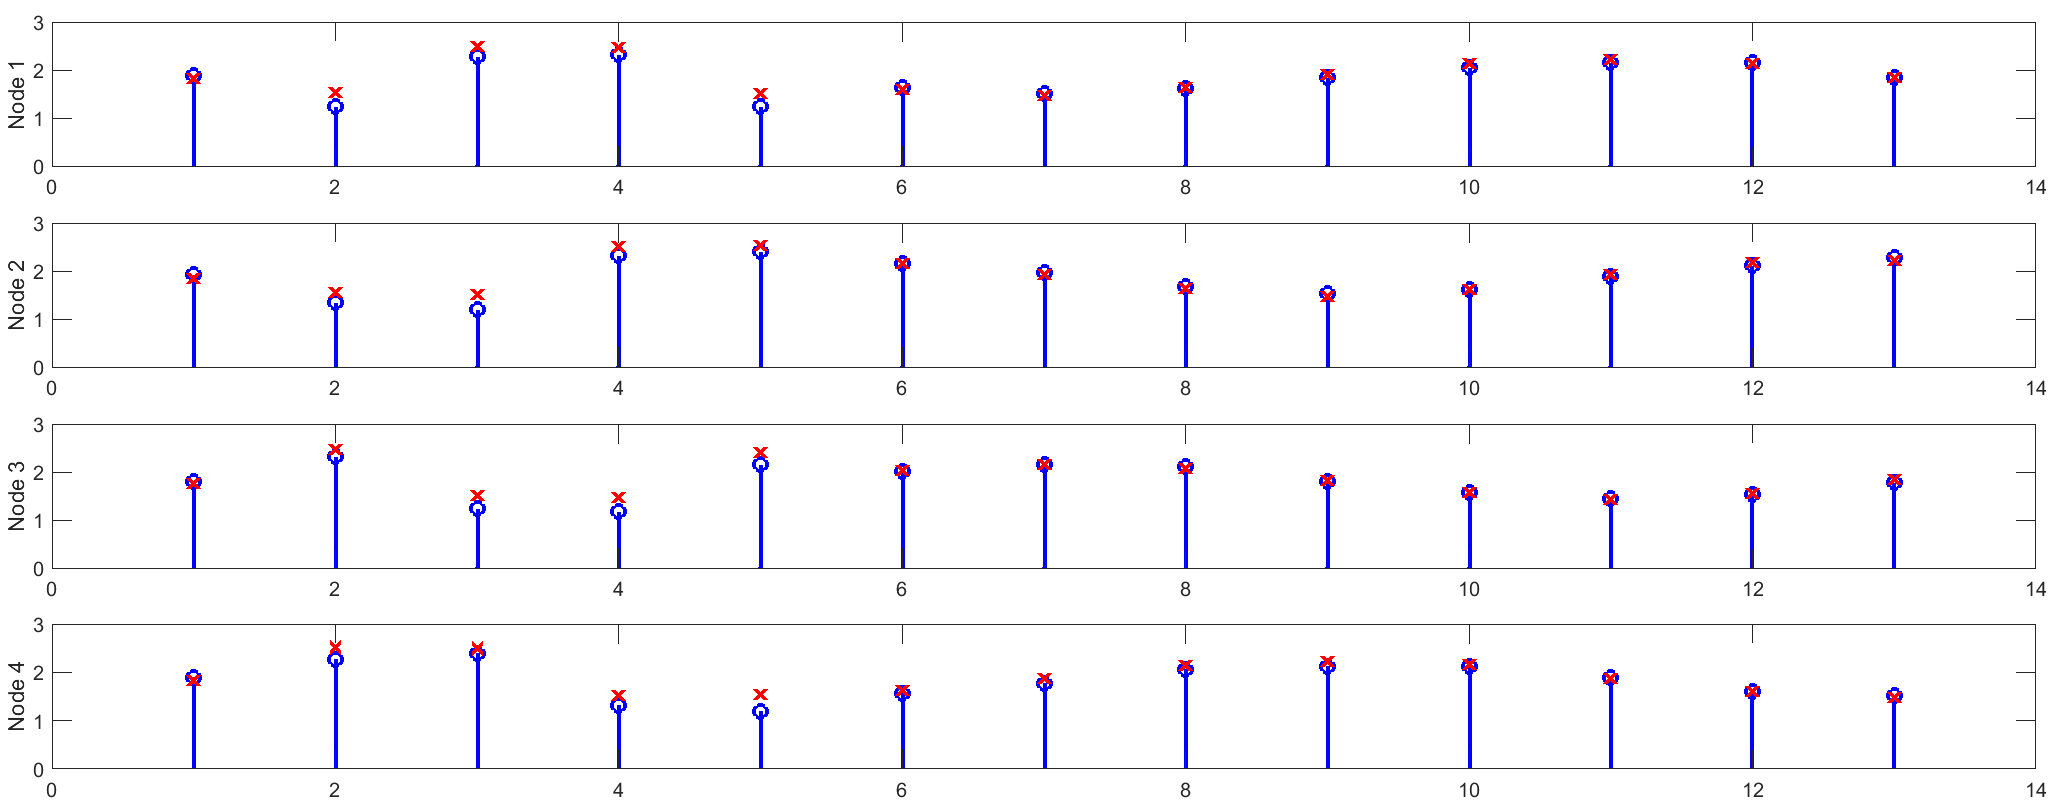
\includegraphics[width=0.9\linewidth]{../Images/Experiments-Results/nodes-estimations.png}
  \decoRule
  \caption[Γραφική αναπαράσταση της εκτίμησης θέσης - πραγματικής απόστασης]{Γραφική αναπαράσταση της εκτίμησης θέσης - πρα\-γμα\-τι\-κής απόστασης (Σύμφωνα με τα δεδομένα του \Tabl{multiple-nodes-est-act-dist}, όπου \textcolor{blue}{o} οι εκτιμήσεις και \textcolor{red}{x} οι πραγματικές αποστάσεις)}
  \label{fig:est-act-dist-figure}
\end{figure}

Από τις παραπάνω μετρήσεις καταλήγουμε σε συνολικό μέσο όρο σφάλματος τα 0.0974 m. Αν διαχωρίσουμε το σφάλμα, με βάση τις εξωτερικές (2-5) και εσωτερικές (1 και 6-13) θέσεις τότε μπορούμε να καταλήξουμε σε δύο επιπλέον σφάλματα. Για τις εξωτερικές ο μέσος όρος των σφαλμάτων είναι τα 0.2230m ενώ για τις εσωτερικές τα 0.0686m. Ο λόγος που συμβαίνει αυτό, σχετίζεται με την παραμόρφωση που προκαλεί ο φακός της κάμερας (με μεγαλύτερες επιδράσεις προς τα άκρα του image plane), και δεν έγινε εφικτό μέσω του calibration να διορθωθεί.

\FigCaptLabelBasedURL{../Images/Experiments-Results/multiple-nodes/combined/low-res/p2.png.low.png}
{Αντιληπτική ικανότητα από κάθε γωνία λήψης για την θέση 2}%
{multiple-nodes-perception}%
<1>

%----------------------------------------------------------------------

\subsection{Εκτίμηση θέσης και απεικόνιση}
Έχοντας συλλέξει τα δεδομένα που αναφέρθηκαν στη \Sect{multiple-nodes-data-collection}, μπορούσε να χρησιμοποιηθεί ο φορμαλισμός που περιγράφηκε στη \Sect{implementation-obj-mult} για την εκτίμηση της θέσης στον τρισδιάστατο χώρο. 

Χρησιμοποιήθηκαν 4 nodes - με ένα από αυτά να αποτελεί ταυτόχρονα χρέη master και worker node - όπου έστελναν στο σύστημα επαναλαμβανόμενα τα ranges και positions του κάθε node που αναφέρθηκαν παραπάνω, με τον τρόπο που περιγράφηκε στο προηγούμενο κεφάλαιο. Αφού το master λάβει τα πακέτα και πραγματοποιήσει την επεξεργασία, χρησιμοποιεί \textbf{geometry\_msgs/Pose} - αποτελεί ένα από τις βασικές μορφές μηνυμάτων για θέση του \Abbr{ROS} - για να γνωστοποιηθεί στο δίκτυο την εκτίμηση της θέση της μπάλας.

Σύμφωνα με τα παραπάνω, στην \Fig{exp-topics-nodes} φαίνονται τα περιεχόμενα των topic κατά την διαδικασία του πειράματος, ενώ στην \Fig{multi-exp-pos-estimations} μπορούμε να δούμε συνδυαστικά τις γραφικές, στις οποίες παρουσιάζονται οι θέσεις που βρισκόταν το αντικείμενο, καθώς και οι εκτιμήσεις της θέσης που τελικά προέκυψαν.

Από τις εκτιμήσεις και τις ακριβής θέσεις, μπορούμε τελικά να υπολογίσουμε το συνολικό σφάλμα του συστήματος. Για το οποίο καταλήγουμε, ότι το συνολικό σφάλμα εκτίμησης θέσης από το σμήνος να είναι τα 0,1159m.

\begin{figure} [H]
	\centering
	% -----------------
    \begin{minipage}{.5\textwidth}
      \centering
      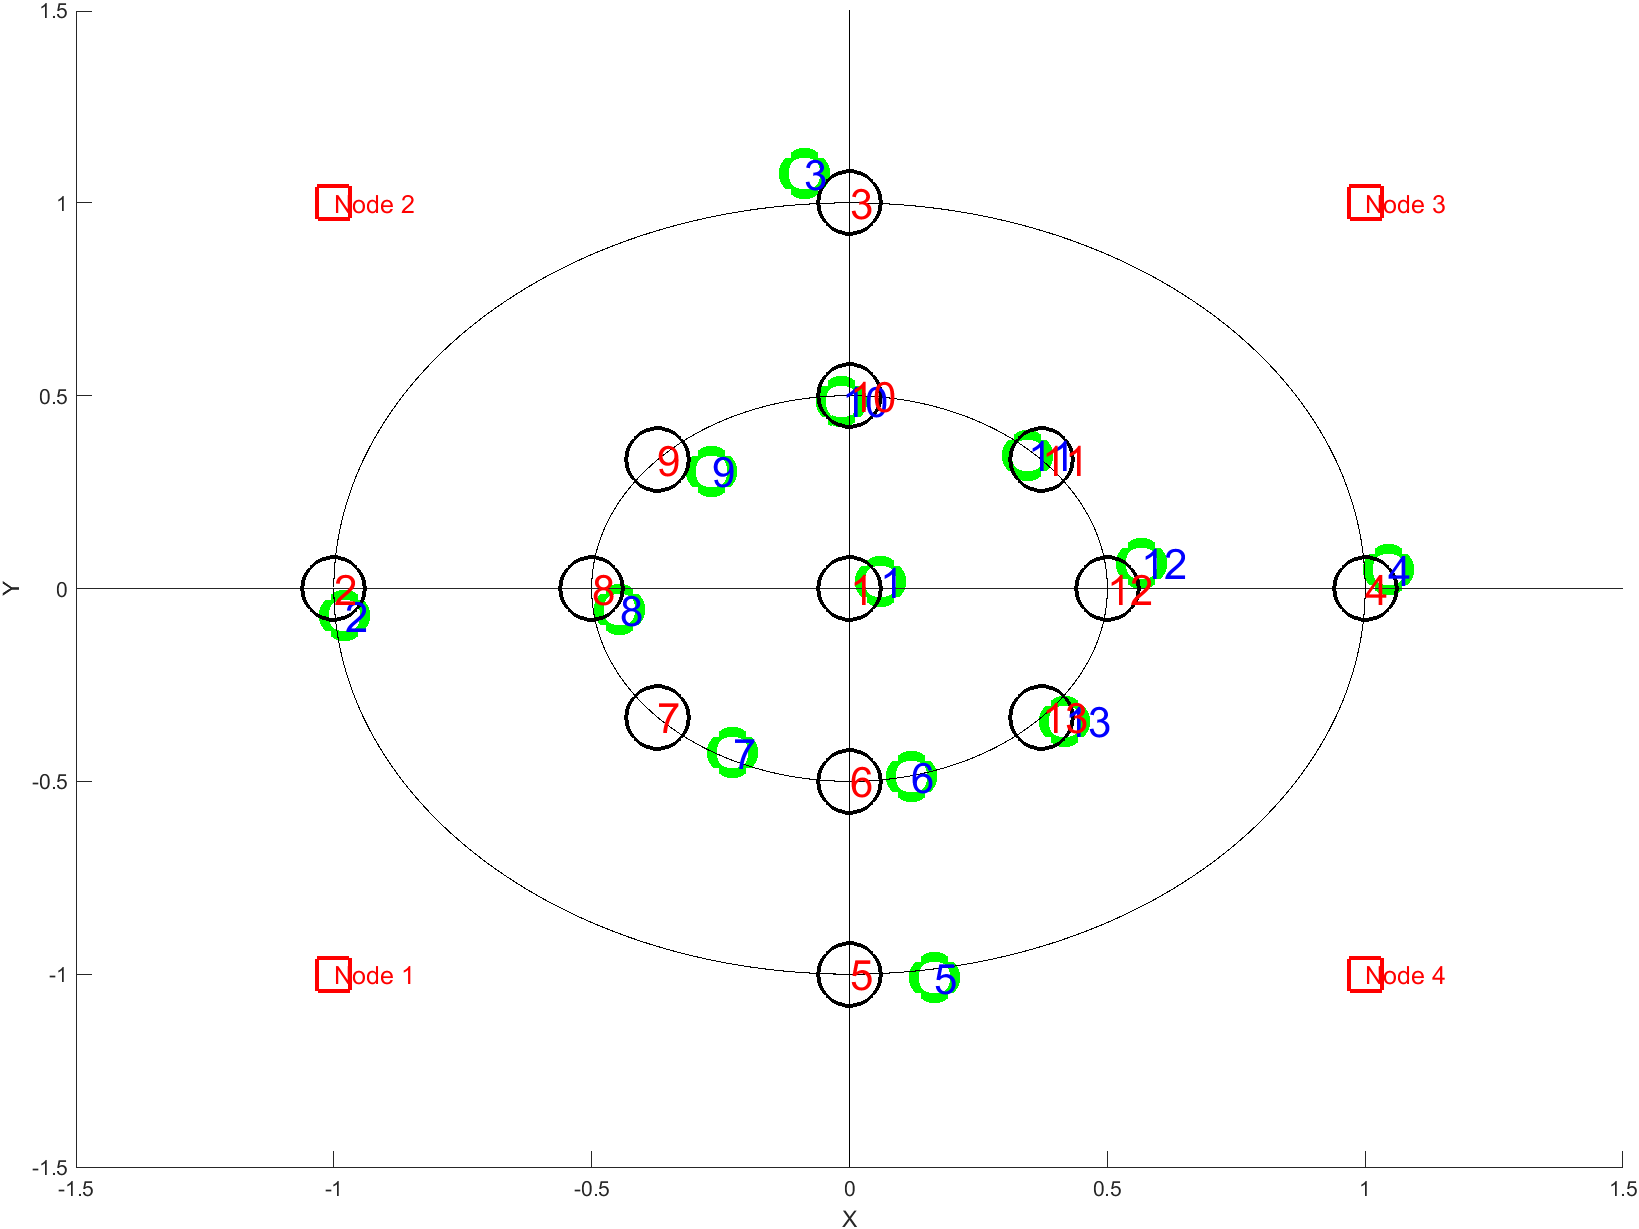
\includegraphics[width=0.9\linewidth]{../Images/Experiments-Results/nodes-pos-with-est-up.png}\\
      {(a) Top View}
    \end{minipage}%
    % -----------------
    \begin{minipage}{.5\textwidth}
      \centering
      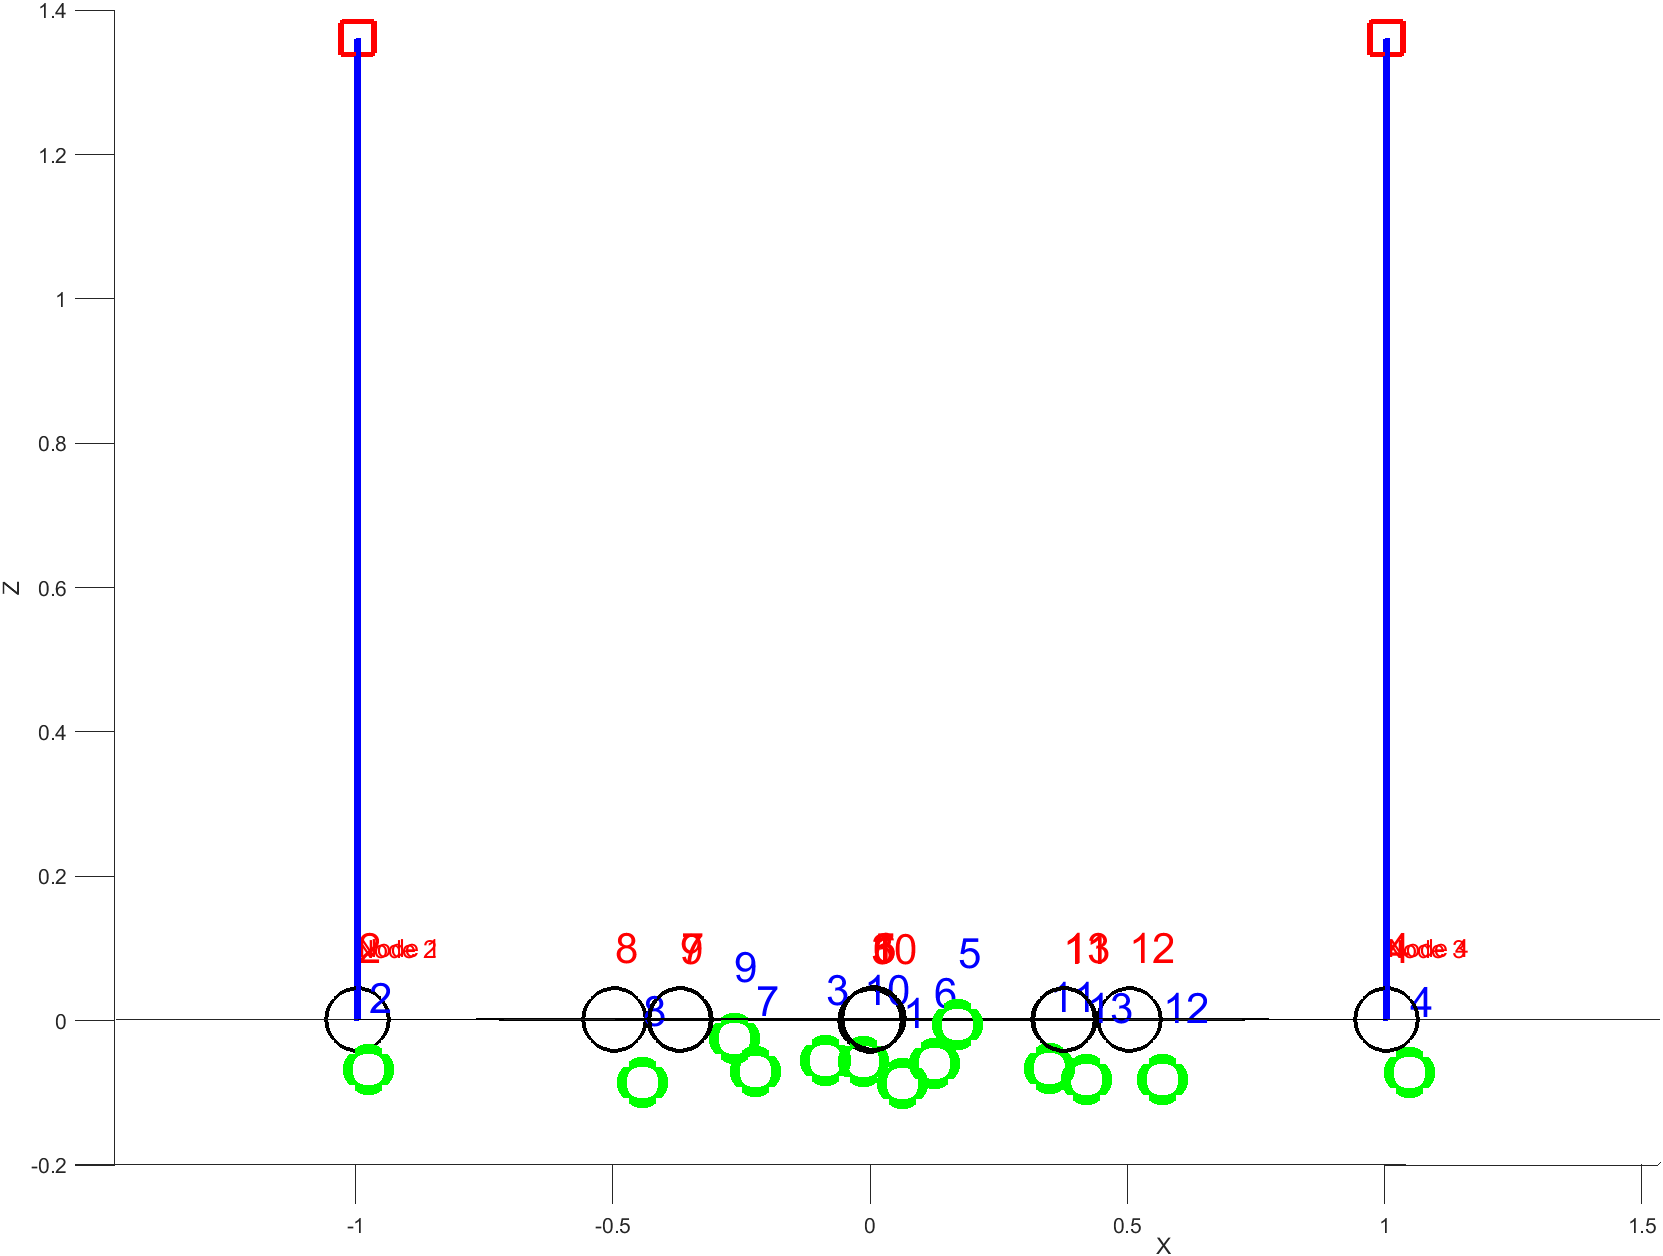
\includegraphics[width=.9\linewidth]{../Images/Experiments-Results/nodes-pos-with-est-side.png}\\
      {(b) Side View}
	  \end{minipage}
	% -----------------
  \begin{minipage}{\textwidth}
    \centering
    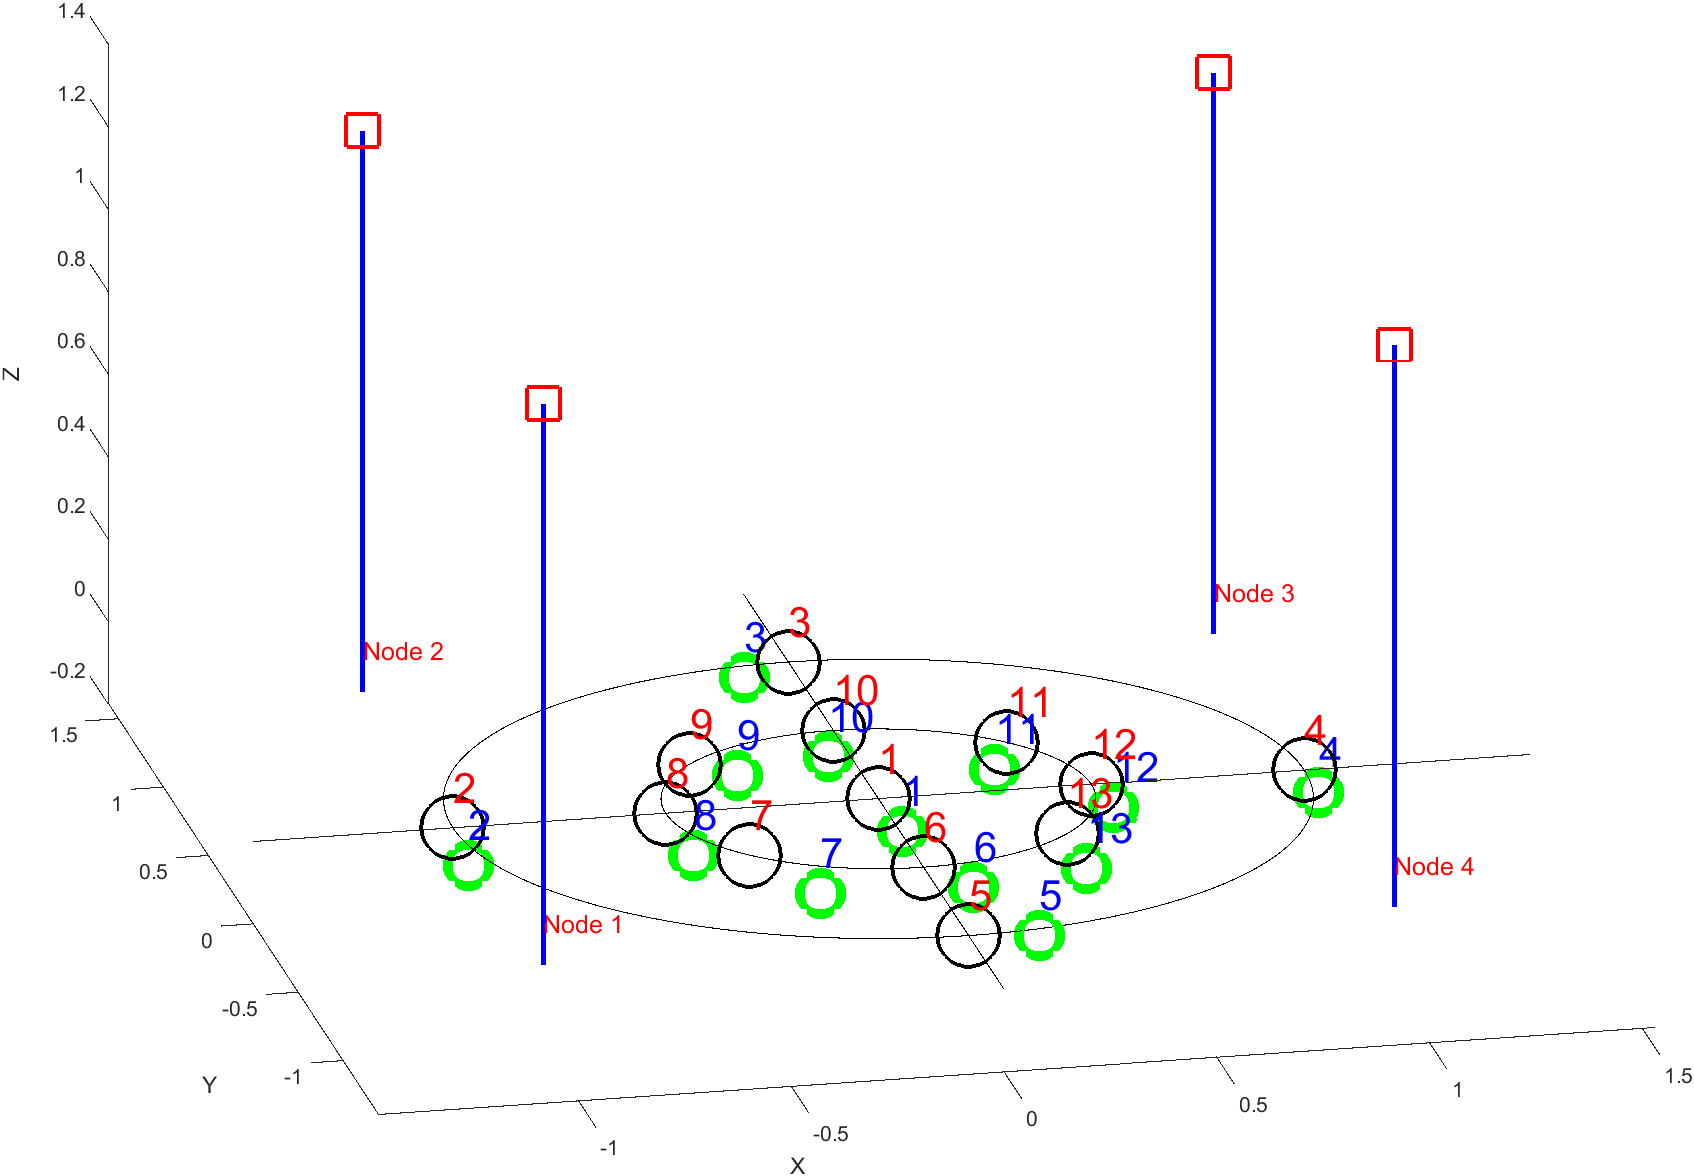
\includegraphics[width=.8\linewidth]{../Images/Experiments-Results/nodes-pos-with-est-angle.png}\\
    {(C) Angled View}
  \end{minipage}
% -----------------
    \hfill \break
    \decoRule
    \caption[Εκτίμηση θέσης του αντικειμένου.]{Εκτίμηση θέσης του αντικειμένου. Με \textcolor{black}{\LARGE$\circ$} είναι οι θέσεις στις οποίες τοποθετήθηκε το αντικείμενο ενώ με \textcolor{green}{\LARGE$\circ$} είναι οι θέσεις που έγινε εκτίμηση ότι βρίσκεται} %\CaptionBasedwithURL{Possible Embedded Linux Systems} 
    \label{fig:multi-exp-pos-estimations}
\end{figure}

\FigCaptLabelBasedURL{../Photos/topics.wr.png}
{Μέρος των εν λειτουργία nodes/topics, καθώς και απεικόνιση των πληροφοριών που αποστέλλουν στα topics τα 4 nodes, μαζί με την εκτίμηση της θέσης από τον master.}%
{exp-topics-nodes}%
<1>

%----------------------------------------------------------------------

\section{Επαλήθευση προσδιορισμού ID}
Όπως αναφέρθηκε στη \Sect{id-estimation} χρησιμοποιούμε την συχνότητα με την οποία αναβοσβήνει το led για τον καθορισμό του ID. Σημαντικός παράγοντας για την επιλογή της συχνότητας είναι το frame-rate της κάμερας με την οποία δειγματοληπτούμε. 

Από το Nyquist–Shannon sampling theorem γνωρίζουμε ότι πρέπει να ισχύει $f_s > 2f_{max}$ μεταξύ της συχνότητας δειγματοληψίας και της μέγιστης συχνότητας σε ένα σήμα. Στην πράξη, είναι συχνό φαινόμενο να επιλέγουμε να διαφέρουν ακόμα και μία τάξη μεγέθους στην παραπάνω ανίσωση. Λόγω των 30fps της κάμερας καταλήγουμε να έχουμε ανά περίπου 33.33ms νέο καρέ, συνεπώς επιλέχθηκε ο χρόνος για τον οποίο θα είναι ενεργοποιημένο το led να είναι τα 70ms ώστε να καταγράφεται από τουλάχιστον 2 καρέ η ενεργοποίηση του. 

Για τις περιόδους ανάλογα με το ID επιλέχθηκαν οι χρόνοι 500ms για ID = 1, 1500ms για ID = 2, 2500ms για ID = 3, κλπ., ώστε να υπάρχει ένα περιθώριο 1000ms για πιθανά σφάλματα μεταξύ των μετρήσεων. 

Η \Fig{id-osci-samples} παρουσιάζει τους παλμούς στους οποίους ενεργοποιείται το led, και κρατάμε αποδεκτό το ID = 1 για durations μεταξύ των παλμών durations <= 1000ms, όμοια για ID = 2 έχουμε 1000ms < duration <= 2000ms, κλπ.

\begin{figure} [H]
	\centering
	% -----------------
    \begin{minipage}{.5\textwidth}
      \centering
      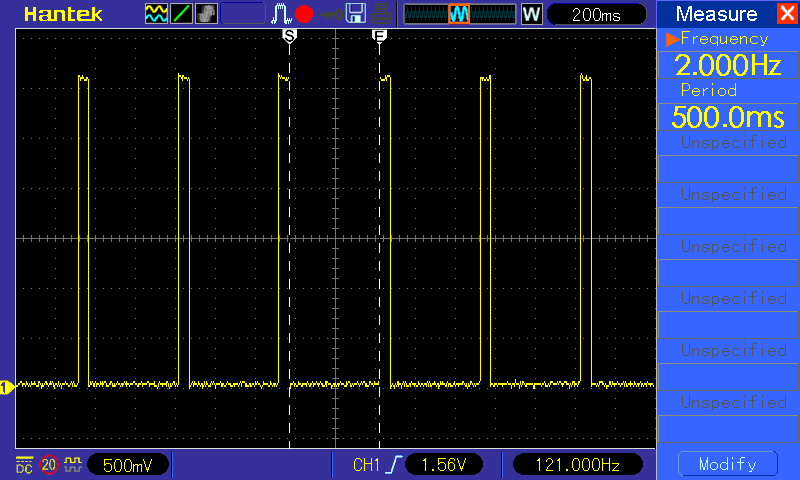
\includegraphics[width=0.9\linewidth]{../Images/Experiments-Results/node-pulses-0_5sec.png}\\
      {(a) Συχνότητα του led για ID = 1}
    \end{minipage}%
    % -----------------
    \begin{minipage}{.5\textwidth}
      \centering
      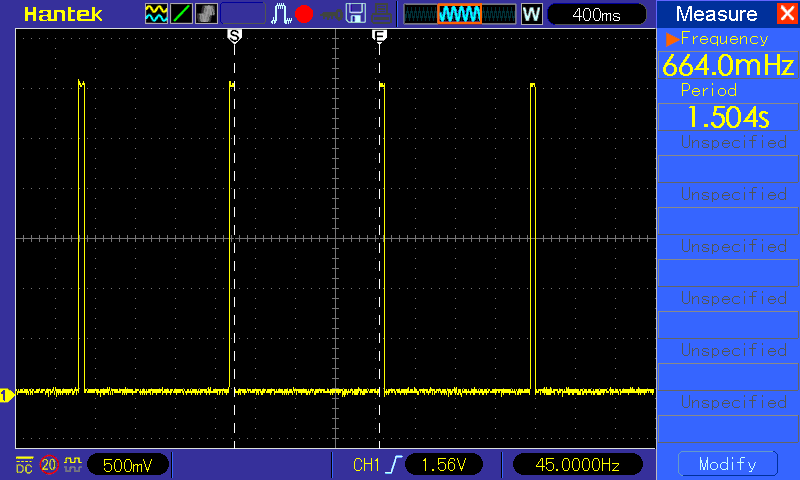
\includegraphics[width=.9\linewidth]{../Images/Experiments-Results/node_pulses_1_5sec.png}\\
      {(b) Συχνότητα του led για ID = 2}
	  \end{minipage}
% -----------------
    \hfill \break
    \decoRule
    \caption[Παράδειγμα δύο εκ των τεσσάρων συχνοτήτων για την λειτουργία του led που επιλέχθηκαν.]{Παράδειγμα δύο εκ των τεσσάρων συχνοτήτων για την λειτουργία του led που επιλέχθηκαν.}%\CaptionBasedwithURL{Possible Embedded Linux Systems} 
    \label{fig:id-osci-samples}
\end{figure}

Τέλος, η \Fig{exp-led-freq} παρουσιάζει στιγμιότυπο κατά την διαδικασία επαλήθευσης της λειτουργίας, στο οποίο παρουσιάζεται τόσο το ID που εκτιμήθηκε όσο και το duration μεταξύ την παλμών.

\FigCaptLabelBasedURL{../Images/Experiments-Results/frequency-analysis.png}
{Στιγμιότυπο της διαδικασίας πείραματος, κατά την διάρκεια καθορισμού του ID του αντικειμένου με βάση την συχνότητα που αναβοσβήνει το led}%
{exp-led-freq}%
<.8>







